\documentclass[a4paper,oneside,12pt]{report}
% Package yang diperlukan
\usepackage[table]{xcolor} % Untuk menggunakan warna
\usepackage{graphicx}      % Untuk memasukkan gambar
\usepackage{titling}       % Untuk kustomisasi halaman judul
\usepackage{geometry}      % Untuk mengatur margin halaman
\usepackage{listings}      % Untuk menampilkan blok kode
\usepackage{float}         % Untuk kontrol penempatan float (seperti gambar)
\usepackage{hyperref}      % Untuk membuat hyperlink (URL, referensi)
\usepackage{indentfirst}   % Untuk memberi indentasi pada paragraf pertama setiap seksi
\usepackage{url}           % Untuk format URL
\usepackage{fancyhdr}      % Untuk kustomisasi header dan footer
\usepackage{tocloft}       % Untuk kustomisasi Daftar Isi
\usepackage{bookmark}      % Untuk manajemen bookmark PDF yang lebih baik
\usepackage{amsmath}       % Untuk notasi matematika
\usepackage[most]{tcolorbox} % Untuk box output terminal

% Paket untuk tabel agar sesuai format referensi
\usepackage{array}
\usepackage{booktabs}
\usepackage{tabularx}
\usepackage{multirow}
\usepackage{colortbl}

% Macro untuk header tabel
\newcommand{\thead}[1]{\textcolor{white}{\textbf{#1}}}

%======================================================================
% PENGATURAN GEOMETRI HALAMAN
%======================================================================
\geometry{left=3cm, right=2.5cm, top=2cm, bottom=2.5cm}
\sloppy

%======================================================================
% PENGATURAN WARNA UNTUK BLOK KODE
%======================================================================
\definecolor{codegreen}{rgb}{0,0.6,0}
\definecolor{codegray}{rgb}{0.5,0.5,0.5}
\definecolor{codepurple}{rgb}{0.58,0,0.82}
\definecolor{backcolour}{rgb}{0.95,0.95,0.92}
\definecolor{darkblue}{rgb}{0,0,0.6}
\definecolor{outputbg}{RGB}{241,245,249}
\definecolor{outputborder}{RGB}{203,213,225}

%======================================================================
% PENGATURAN BLOK KODE (LISTINGS)
%======================================================================
\lstdefinestyle{commonstyle}{
    backgroundcolor=\color{backcolour},
    breakatwhitespace=false,
    breaklines=true,
    captionpos=b,
    keepspaces=true,
    numbers=left,
    numbersep=5pt,
    showspaces=false,
    showstringspaces=false,
    showtabs=false,
    tabsize=2,
    frame=single,
    basicstyle=\ttfamily\footnotesize,
    numberstyle=\tiny\color{codegray},
    columns=flexible,
    postbreak=\mbox{\textcolor{red}{$\hookrightarrow$}\space},
    breakindent=0pt,
    breakautoindent=false
}

\lstdefinestyle{pythonstyle}{
    style=commonstyle,
    language=Python,
    commentstyle=\color{codegreen},
    keywordstyle=\color{darkblue},
    stringstyle=\color{codepurple},
    emph={import,from,class,def,for,while,if,else,elif,try,except,finally,as,lambda,return},
    emphstyle=\color{darkblue}
}

% Box Format Output / Terminal Box (Verbatim via tcblisting)
\newtcblisting{outputbox}{
    enhanced,
    colback=outputbg,
    colframe=outputborder,
    boxrule=0.6pt,
    arc=1.2mm,
    left=3mm,
    right=3mm,
    top=1.2mm,
    bottom=1.2mm,
    listing only,
    listing options={
        basicstyle=\ttfamily\footnotesize,
        breaklines=true,
        numbers=none,
        showstringspaces=false
    }
}

\newcommand{\screenshotimage}[4][0.88\textwidth]{%
    \begin{figure}[H]
        \centering
        \includegraphics[width=#1]{#2}
        \caption{#3}
        \label{fig:#4}
    \end{figure}
}

%======================================================================
% PENGATURAN LAIN-LAIN
%======================================================================
\renewcommand{\figurename}{Gambar}
\renewcommand{\thefigure}{\arabic{figure}}
\renewcommand{\tablename}{Tabel}

\hypersetup{
    colorlinks=true,
    linkcolor=black,
    filecolor=black,
    urlcolor=black,
    citecolor=black,
    pdftitle={Laporan Praktikum Penambangan Data Pertemuan IV},
    pdfpagemode=FullScreen,
    breaklinks=true
}

\pagestyle{fancy}
\fancyhf{}
\fancyfoot[C]{\thepage}
\renewcommand{\headrulewidth}{0pt}

\fancypagestyle{plain}{
    \fancyhf{}
    \fancyfoot[C]{\thepage}
    \renewcommand{\headrulewidth}{0pt}
}

%======================================================================
% PENGATURAN STRUKTUR BAB DAN DAFTAR ISI
%======================================================================
\renewcommand{\contentsname}{Daftar Isi}
\renewcommand{\bibname}{Daftar Pustaka}

\renewcommand{\thechapter}{}
\renewcommand{\chaptername}{}

\renewcommand{\thesection}{\arabic{chapter}.\arabic{section}}
\renewcommand{\thesubsection}{\thesection.\arabic{subsection}}

\setcounter{secnumdepth}{2}
\setcounter{tocdepth}{2}

\renewcommand{\cftchapdotsep}{\cftdotsep}
\renewcommand{\cftchapleader}{\cftdotfill{\cftchapdotsep}}
\setlength{\cftchapindent}{0em}
\setlength{\cftsecindent}{2em}
\setlength{\cftsubsecindent}{4em}
\setlength{\cftchapnumwidth}{0em}
\setlength{\cftsecnumwidth}{2.5em}
\setlength{\cftsubsecnumwidth}{3.2em}
\renewcommand{\cftchappresnum}{}
\renewcommand{\cftchapaftersnum}{}

%======================================================================
% AWAL DOKUMEN
%======================================================================
\begin{document}

\newgeometry{left=3cm, right=2.5cm, top=2.5cm, bottom=3cm}
\begin{titlingpage}
\begin{center}
\vspace*{0.5cm}
{\large \textbf{\MakeUppercase{Laporan Praktikum}}} \\[0.4cm]
{\large \textbf{\MakeUppercase{Praktikum Penambangan Data}}} \\[0.4cm]
{\large \textbf{\MakeUppercase{Pertemuan IV}}} \\[0.4cm]
{\large \textbf{\MakeUppercase{Regression}}} \\[1.5cm]


\includegraphics[height=7cm]{lambang ugm.png} \\[1cm]

{\normalsize \textbf{Disusun oleh:}} \\[0.4cm]
\begin{tabular}{@{}l l @{}}
  \textbf{Nama}           & : Januarsyah Akbar \\
  \textbf{NIM}            & : 24/535846/SV/24314 \\
  \textbf{Kelas}          & : B2 \\
  \textbf{Dosen Pengampu} & : Dr. Ganjar Alfian, S.T., M.Eng. \\
                          & \phantom{:} Dr. Imam Fahrurrozi, S.T., M.Cs.
\end{tabular} \\[1.2cm]

{\normalsize \textbf{PROGRAM STUDI D-IV}} \\[0.2cm]
{\normalsize \textbf{TEKNOLOGI REKAYASA PERANGKAT LUNAK}} \\[0.2cm]
{\normalsize \textbf{DEPARTEMEN TEKNIK ELEKTRO DAN INFORMATIKA}} \\[0.2cm]
{\normalsize \textbf{SEKOLAH VOKASI}} \\[0.2cm]
{\normalsize \textbf{UNIVERSITAS GADJAH MADA}} \\[0.2cm]
{\normalsize \textbf{YOGYAKARTA}} \\[0.2cm]
{\normalsize \textbf{2026}} \\[1.2cm]
\end{center}
\end{titlingpage}
\restoregeometry

\thispagestyle{empty}
\clearpage
\stepcounter{page}
\thispagestyle{empty}

% --- Daftar Isi ---
\addcontentsline{toc}{chapter}{Daftar Isi}
\tableofcontents
\clearpage

\pagenumbering{arabic}
\setcounter{page}{3}

%======================================================================
% BAB I: TUJUAN PRAKTIKUM
%======================================================================
\chapter[Tujuan Praktikum]{Tujuan Praktikum}
Tujuan pelaksanaan praktikum pada Pertemuan IV adalah sebagai berikut:
\begin{enumerate}
    \item Mahasiswa mampu memahami konsep dasar regresi dalam memodelkan variabel target bertipe numerik atau kontinu.
    \item Mahasiswa mengetahui prinsip kerja algoritma regresi, khususnya Linear Regression, Decision Tree Regression, dan Random Forest Regression.
    \item Mahasiswa dapat menerapkan algoritma regresi untuk membangun model estimasi nilai kontinu pada dataset riil.
    \item Mahasiswa mampu mengevaluasi performa model regresi menggunakan metrik Root Mean Squared Error (RMSE), Coefficient of Determination ($R^2$), serta nilai koefisien korelasi Pearson ($R$).
\end{enumerate}
\clearpage

%======================================================================
% BAB II: DASAR TEORI
%======================================================================
\chapter{Dasar Teori}

\section{Regresi}
Regresi merupakan salah satu metode analisis statistik dalam ranah \textit{supervised learning}. Teknik ini digunakan untuk memodelkan hubungan matematis antara satu atau lebih variabel independen (fitur prediktor) dengan variabel dependen (target) yang bersifat numerik kontinu \cite{ref4}. Tujuan utama regresi adalah memahami pola ketergantungan antarvariabel, memprediksi besaran numerik di masa depan, dan mengukur elastisitas pengaruh masing-masing fitur terhadap output akhir. Contoh penerapan regresi mencakup estimasi harga properti, proyeksi penjualan retail, prediksi konsumsi energi, dan penilaian valuasi kendaraan bermotor.

\section{Algoritma Regresi}
Tiga algoritma regresi yang dipelajari pada praktikum ini memiliki karakteristik matematis dan struktur pemodelan yang berlainan \cite{ref6}:

\begin{enumerate}
    \item \textbf{Linear Regression}: \\
    Linear Regression memodelkan relasi antara fitur dan target melalui asumsi garis lurus atau bidang datar (\textit{hyperplane}) linear. Model berusaha menentukan kombinasi bobot koefisien yang meminimalkan akumulasi kuadrat selisih antara nilai aktual dan estimasi menggunakan metode kuadrat terkecil (\textit{Ordinary Least Squares}). Persamaan dasar Linear Regression dirumuskan sebagai:
    \begin{equation}
        y = b_0 + b_1 x_1 + b_2 x_2 + \dots + b_n x_n
    \end{equation}
    dengan $b_0$ menyatakan nilai intercept (konstanta dasar), $b_n$ merupakan bobot koefisien regresi untuk fitur ke-$n$, dan $y$ adalah nilai prediksi target. Model linear memiliki keunggulan komputasi yang sangat cepat serta interpretasi bobot yang jelas, namun kurang fleksibel dalam menangkap pola non-linear dan rentan terdistorsi oleh keberadaan data pencilan (\textit{outliers}).

    \item \textbf{Decision Tree Regression}: \\
    Decision Tree Regression membagi ruang sampel secara berulang (\textit{recursive binary splitting}) ke dalam wilayah-wilayah yang lebih homogen. Titik pemisahan (\textit{split point}) pada setiap simpul internal ditentukan berdasarkan penurunan nilai galat terbesar, umumnya memakai kriteria \textit{Mean Squared Error} (MSE). Setiap daun (\textit{leaf node}) merepresentasikan nilai estimasi berupa rata-rata target dari data yang masuk ke wilayah tersebut. Model ini mampu memetakan interaksi non-linear yang rumit tanpa menuntut normalisasi fitur, namun rentan mengalami \textit{overfitting} jika kedalaman pohon tidak dibatasi melalui parameter pemangkasan.

    \item \textbf{Random Forest Regression}: \\
    Random Forest Regression merupakan algoritma pembelajaran ansambel (\textit{ensemble learning}) berbasis penggabungan pohon keputusan acak. Melalui teknik \textit{bootstrap aggregating} (\textit{bagging}), algoritma melatih ratusan pohon keputusan independen menggunakan sampel acak berulang serta subset fitur acak pada setiap percabangan simpul. Estimasi akhir diperoleh dengan merata-ratakan nilai prediksi dari seluruh pohon di dalam hutan ansambel:
    \begin{equation}
        \hat{y} = \frac{1}{B}\sum_{b=1}^B T_b(x)
    \end{equation}
    Mekanisme rata-rata ini menekan varians model secara drastis tanpa menambah bias, sehingga Random Forest menghasilkan prediksi yang jauh lebih akurat dan stabil dibandingkan pohon keputusan tunggal.
\end{enumerate}

\section{Metrik Evaluasi Regresi}
Kualitas estimasi model regresi diukur menggunakan metrik statistik khusus nilai kontinu \cite{ref4}:

\begin{enumerate}
    \item \textbf{Root Mean Squared Error (RMSE)}: \\
    RMSE mengukur akar kuadrat dari rata-rata selisih kuadrat antara nilai prediksi dengan nilai aktual. Karena nilai selisih dikuadratkan terlebih dahulu sebelum ditarik akar, RMSE memberikan bobot penalti yang lebih tegas terhadap galat berukuran besar. Satuan RMSE setara dengan satuan variabel target sehingga mempermudah pembacaan deviasi riil.
    \begin{equation}
        \text{RMSE} = \sqrt{\frac{1}{n}\sum_{i=1}^n (y_i - \hat{y}_i)^2}
    \end{equation}

    \item \textbf{Coefficient of Determination ($R^2$)}: \\
    Nilai $R^2$ mengukur proporsi variabilitas variabel target yang mampu diterangkan oleh fitur-fitur di dalam model. Nilai $R^2$ bergerak pada rentang 0 hingga 1. Nilai yang mendekati angka 1 menandakan bahwa model mampu menangkap struktur sebaran data dengan presisi tinggi.
    \begin{equation}
        R^2 = 1 - \frac{\sum_{i=1}^n (y_i - \hat{y}_i)^2}{\sum_{i=1}^n (y_i - \bar{y})^2}
    \end{equation}

    \item \textbf{Koefisien Korelasi Pearson ($R$)}: \\
    Koefisien korelasi $R$ mengukur kekuatan hubungan linier antara nilai target aktual dengan nilai hasil prediksi model. Nilai $R$ bernilai antara $-1$ hingga $+1$. Nilai positif mendekati $+1$ membuktikan bahwa peningkatan nilai aktual diimbangi oleh peningkatan nilai estimasi model secara konsisten.
    \begin{equation}
        R = \frac{\sum_{i=1}^n (y_i - \bar{y})(\hat{y}_i - \bar{\hat{y}})}{\sqrt{\sum_{i=1}^n (y_i - \bar{y})^2 \sum_{i=1}^n (\hat{y}_i - \bar{\hat{y}})^2}}
    \end{equation}
\end{enumerate}
\clearpage

%======================================================================
% BAB III: HASIL DAN PEMBAHASAN
%======================================================================
\chapter{Hasil dan Pembahasan}

\section{Langkah Percobaan (KC House Data)}
Percobaan modul memfokuskan pemodelan regresi harga rumah pada dataset \textit{House Sales in King County, USA}. Seluruh tahapan disusun dan dieksekusi secara terstruktur pada Google Colab.

\subsection{Import Pustaka dan Pemuatan Dataset}
Pustaka dasar komputasi (Pandas, NumPy, Matplotlib, Seaborn) dimuat bersama modul regresi dan evaluasi dari Scikit-Learn. Dataset berformat CSV diunduh langsung dari tautan repositori daring.

\begin{lstlisting}[style=pythonstyle, caption=Import Pustaka dan Pembacaan Dataset KC House Data]
import pandas as pd
import matplotlib.pyplot as plt
import numpy as np
import seaborn as sns

from sklearn.linear_model import LinearRegression
from sklearn.model_selection import train_test_split
from sklearn.metrics import mean_squared_error, r2_score
from sklearn.tree import DecisionTreeRegressor
from sklearn.ensemble import RandomForestRegressor

df = pd.read_csv('https://raw.githubusercontent.com/ganjar87/data_science_practice/main/kc_house_data.csv')
\end{lstlisting}

Dataset tersimpan ke dalam variabel \texttt{df} dengan volume sebesar 21.613 baris observasi transaksi penjualan rumah dan 21 kolom atribut properti.

\subsection{Exploratory Data Analysis (EDA)}
Inspeksi data dilakukan guna memeriksa struktur nilai, sebaran frekuensi, keberadaan data kosong, dan relasi linear antarfitur.

\begin{enumerate}
    \item \textbf{Inspeksi Baris Pertama dan Terakhir}: \\
    Perintah \texttt{df.head()} dan \texttt{df.tail()} menampilkan lima data teratas dan terbawah. Kolom dataset mencakup identitas rumah (\texttt{id}), tanggal penjualan (\texttt{date}), variabel target harga (\texttt{price}), jumlah kamar tidur (\texttt{bedrooms}), kamar mandi (\texttt{bathrooms}), luas bangunan (\texttt{sqft\_living}), luas tanah (\texttt{sqft\_lot}), lantai (\texttt{floors}), tepi laut (\texttt{waterfront}), kualitas pemandangan (\texttt{view}), kondisi fisik (\texttt{condition}), tingkat kualitas konstruksi (\texttt{grade}), koordinat lokasi (\texttt{lat}, \texttt{long}), serta spesifikasi lingkungan sekitar (\texttt{sqft\_living15}, \texttt{sqft\_lot15}). Hasil eksekusi pada Google Colab disajikan pada Gambar \ref{fig:colab-eda-head}.

    \screenshotimage{gambar/colab-eda-head.png}{Output Lima Baris Pertama dan Terakhir KC House Data di Google Colab}{colab-eda-head}

    \item \textbf{Statistik Deskriptif Dataset}: \\
    Fungsi \texttt{df.describe()} menyajikan ringkasan statistik dari 21.613 unit rumah. Harga jual (\texttt{price}) memiliki nilai rata-rata sebesar 540.088 USD, nilai minimum 75.000 USD, kuartil bawah (Q1) 321.950 USD, median 450.000 USD, kuartil atas (Q3) 645.000 USD, dan harga maksimum menyentuh 7.700.000 USD. Standar deviasi harga yang mencapai 367.127 USD menandakan variasi nilai properti yang lebar. Tampilan statistik deskriptif pada Google Colab disajikan pada Gambar \ref{fig:colab-eda-describe}.

    \screenshotimage{gambar/colab-eda-describe.png}{Output Ringkasan Statistik Deskriptif KC House Data di Google Colab}{colab-eda-describe}

    \item \textbf{Visualisasi Histogram Fitur Numerik}: \\
    Perintah \texttt{df.hist(figsize=(10,10))} memetakan distribusi sebaran data seluruh fitur, sebagaimana disajikan pada Gambar \ref{fig:hist_kc_house}.

    \screenshotimage{gambar/hist_kc_house.png}{Histogram Distribusi Seluruh Fitur Numerik KC House Data}{hist_kc_house}

    Kurva harga rumah (\texttt{price}), luas bangunan (\texttt{sqft\_living}), dan luas tanah (\texttt{sqft\_lot}) memperlihatkan pola miring ke kanan (\textit{right-skewed distribution}), di mana sebagian besar hunian berada pada rentang harga menengah ke bawah dengan sejumlah kecil transaksi bernilai sangat tinggi.

    \item \textbf{Korelasi Antarfitur Numerik}: \\
    Pemeriksaan keterkaitan linear dilakukan lewat matriks korelasi \texttt{df.corr(numeric\_only=True)}. Gambar \ref{fig:colab-eda-corr} memperlihatkan tabel matriks korelasi di Google Colab, sedangkan Gambar \ref{fig:corr_kc_house} menampilkan visualisasi matriks korelasi Pearson.

    \screenshotimage{gambar/colab-eda-corr.png}{Output Tabel Matriks Korelasi Numerik KC House Data di Google Colab}{colab-eda-corr}

    \screenshotimage{gambar/corr_kc_house.png}{Matriks Korelasi Pearson Fitur Numerik KC House Data}{corr_kc_house}

    Variabel yang memiliki korelasi positif paling tinggi terhadap harga adalah luas ruang tinggal (\texttt{sqft\_living}, $r = 0.70$), kualitas kelas konstruksi (\texttt{grade}, $r = 0.67$), luas lantai atas (\texttt{sqft\_above}, $r = 0.61$), dan luas ruang tinggal 15 tetangga terdekat (\texttt{sqft\_living15}, $r = 0.59$).

    \item \textbf{Pengecekan Nilai Hilang dan Atribut Kategorikal}: \\
    Eksekusi \texttt{df.isnull().sum()} menghasilkan angka 0 untuk seluruh kolom, membuktikan dataset bersih dari data kosong. Selanjutnya, penyaringan tipe data non-angka menunjukkan bahwa seluruh fitur prediktor telah berbentuk numerik kontinu maupun diskret.
\end{enumerate}

\begin{lstlisting}[style=pythonstyle, caption=Pengecekan Missing Value dan Tipe Fitur Kategorikal]
df_X = df.drop(['id', 'date', 'price'], axis=1)
y = df['price']
print("Missing values total:", df.isnull().sum().sum())
cats = df_X.select_dtypes(include=['object', 'bool']).columns
print("Kolom kategorikal:", cats)
\end{lstlisting}

\screenshotimage[0.78\textwidth]{gambar/colab-eda-null.png}{Output Pengecekan Missing Values Dataset KC House di Google Colab}{colab-eda-null}

\subsection{Pemodelan Regresi dan Evaluasi (KC House Data)}
Fitur prediktor dibentuk dengan membuang kolom non-informatif (\texttt{id} dan \texttt{date}) serta kolom target (\texttt{price}). Data dikonversi ke array numerik dan dibagi menjadi 70\% data latih (15.129 baris) dan 30\% data uji (6.484 baris) menggunakan \texttt{random\_state=42}.

\begin{enumerate}
    \item \textbf{Linear Regression} \\
    Model Linear Regression diinisialisasi dan dilatih menggunakan metode \textit{Ordinary Least Squares}.
\begin{lstlisting}[style=pythonstyle, caption=Pelatihan dan Evaluasi Linear Regression pada KC House]
X = df_X.astype(float).values
y = df['price'].astype(float).values

X_train, X_test, y_train, y_test = train_test_split(X, y, test_size=0.3, random_state=42)
reg = LinearRegression()
reg.fit(X_train, y_train)

y_pred = reg.predict(X_test)
mse = mean_squared_error(y_test, y_pred)
rmse = np.sqrt(mse)
r2 = r2_score(y_test, y_pred)

print('Train R2:', reg.score(X_train, y_train))
print('Test R2 :', r2)
print('RMSE    :', rmse)
print('Intercept:', reg.intercept_)
\end{lstlisting}

\screenshotimage[0.72\textwidth]{gambar/colab-model-lr-output.png}{Output Evaluasi Model Linear Regression KC House di Google Colab}{colab-model-lr-output}

Skor koefisien determinasi data latih ($0.6995$) dan data uji ($0.6995$) bernilai identik, membuktikan model linear berada dalam kondisi stabil tanpa gejala overfitting. Namun, nilai RMSE sebesar 208.296,73 USD masih tergolong besar karena relasi harga rumah terhadap kombinasi fitur lingkungan memiliki kecenderungan non-linear. Gambar \ref{fig:bar_comp_lr} memperlihatkan diagram perbandingan antara nilai aktual dan estimasi Linear Regression pada 50 sampel pengujian awal.

\screenshotimage{gambar/bar_comp_lr.png}{Diagram Batang Perbandingan Nilai Riil vs Prediksi Linear Regression (50 Sampel)}{bar_comp_lr}

    \item \textbf{Decision Tree Regression} \\
    Pohon keputusan dibangun menggunakan batasan kedalaman maksimum \texttt{max\_depth=10} untuk membatasi kompleksitas simpul percabangan.
\begin{lstlisting}[style=pythonstyle, caption=Pelatihan dan Evaluasi Decision Tree Regression pada KC House]
dt = DecisionTreeRegressor(max_depth=10, random_state=42)
dt.fit(X_train, y_train)

y_pred_dt = dt.predict(X_test)
mse_dt = mean_squared_error(y_test, y_pred_dt)
rmse_dt = np.sqrt(mse_dt)
r2_dt = r2_score(y_test, y_pred_dt)

print('Train R2:', dt.score(X_train, y_train))
print('Test R2 :', r2_dt)
print('RMSE    :', rmse_dt)
\end{lstlisting}

\screenshotimage[0.72\textwidth]{gambar/colab-model-dt-output.png}{Output Evaluasi Model Decision Tree Regression KC House di Google Colab}{colab-model-dt-output}

Pembatasan kedalaman menghasilkan nilai $R^2$ data latih sebesar $0.9185$ dan $R^2$ data uji sebesar $0.7586$. Nilai RMSE berhasil ditekan menjadi 186.675,48 USD (turun sekitar 21.600 USD dibanding Linear Regression). Struktur pemisahan hierarkis mampu memetakan interaksi wilayah dan kondisi rumah secara lebih fleksibel. Gambar \ref{fig:bar_comp_dt} menunjukkan profil diagram batang Decision Tree yang lebih mendekati batang nilai aktual.

\screenshotimage{gambar/bar_comp_dt.png}{Diagram Batang Perbandingan Nilai Riil vs Prediksi Decision Tree (50 Sampel)}{bar_comp_dt}

    \item \textbf{Random Forest Regression} \\
    Model ensemble Random Forest menggabungkan banyak pohon keputusan acak melalui prinsip agregasi rata-rata (\textit{bagging}).
\begin{lstlisting}[style=pythonstyle, caption=Pelatihan dan Evaluasi Random Forest Regression pada KC House]
rf = RandomForestRegressor(random_state=42)
rf.fit(X_train, y_train)

y_pred_rf = rf.predict(X_test)
mse_rf = mean_squared_error(y_test, y_pred_rf)
rmse_rf = np.sqrt(mse_rf)
r2_rf = r2_score(y_test, y_pred_rf)

print('Train R2:', rf.score(X_train, y_train))
print('Test R2 :', r2_rf)
print('RMSE    :', rmse_rf)
\end{lstlisting}

\screenshotimage[0.72\textwidth]{gambar/colab-model-rf-output.png}{Output Evaluasi Model Random Forest Regression KC House di Google Colab}{colab-model-rf-output}

Random Forest mencatatkan performa paling unggul di seluruh parameter uji. Nilai $R^2$ data uji melonjak ke angka $0.8540$ dan nilai RMSE terpangkas menjadi 145.205,69 USD. Hal ini mengonfirmasi bahwa perpaduan multi-pohon acak efektif menekan varians kesalahan prediksi individu pohon. Gambar \ref{fig:bar_comp_rf} memperlihatkan diagram batang prediksi Random Forest yang paling selaras dengan nilai riil pasar.

\screenshotimage{gambar/bar_comp_rf.png}{Diagram Batang Perbandingan Nilai Riil vs Prediksi Random Forest (50 Sampel)}{bar_comp_rf}
\end{enumerate}

\subsection{Rekapitulasi Evaluasi Model Percobaan}
Hasil perbandingan metrik performa ketiga model pada data uji KC House dirangkum pada Gambar \ref{fig:colab-kc-eval-table} dan visualisasi diagram batang pada Gambar \ref{fig:kc_house_eval_comp}.

\screenshotimage[0.78\textwidth]{gambar/colab-kc-eval-table.png}{Tabel Ringkasan Evaluasi Model Regresi KC House Data di Google Colab}{colab-kc-eval-table}

\screenshotimage{gambar/kc_house_eval_comp.png}{Perbandingan Metrik RMSE dan $R^2$ Ketiga Algoritma Regresi pada KC House Data}{kc_house_eval_comp}

\clearpage

%======================================================================
% BAGIAN TUGAS DAN ANALISIS
%======================================================================
\section{Tugas dan Analisis (Car Price Prediction Dataset)}
Eksperimen tugas menerapkan ketiga algoritma regresi untuk mengestimasi harga jual mobil di pasar Amerika Serikat menggunakan dataset \textit{Car Price Prediction}.

\subsection{Tujuan Penggunaan Dataset dan Definisi Atribut}
\begin{enumerate}
    \item \textbf{Tujuan Penggunaan Dataset}: \\
    Dataset ini digunakan oleh analis industri otomotif untuk memodelkan faktor-faktor teknis dan preferensi rancang bangun yang menentukan harga pasar suatu kendaraan. Model regresi yang dihasilkan membantu pabrikan menentukan strategi spesifikasi mesin, dimensi bodi, serta segmentasi harga yang tepat guna bersaing di pasar global. Hasil pembacaan dataset serta pemeriksaan dimensi awal di Google Colab disajikan pada Gambar \ref{fig:colab-car-head}.

    \screenshotimage{gambar/colab-car-head.png}{Pemuatan Dataset Mobil dan Cuplikan Data di Google Colab}{colab-car-head}

    \item \textbf{Definisi Atribut Input dan Output}: \\
    Rincian 26 kolom atribut penyusun dataset dipetakan pada Tabel \ref{tab:car_attributes}.
\end{enumerate}

\begin{table}[H]
\centering
\caption{Definisi Atribut Dataset Car Price Prediction}
\label{tab:car_attributes}
\vspace{0.2cm}
\footnotesize
\rowcolors{2}{gray!10}{white}
\begin{tabularx}{\textwidth}{l l l X}
\toprule
\rowcolor{darkblue}
\thead{Nama Atribut} & \thead{Tipe Data} & \thead{Peran} & \thead{Keterangan} \\
\midrule
\texttt{car\_ID} & Numerik & Identitas & Nomor unik indeks mobil (dieliminasi dari model). \\
\texttt{CarName} & Teks & Identitas & Nama merek dan tipe mobil (dieliminasi dari model). \\
\texttt{symboling} & Numerik & Input & Tingkat risiko asuransi mobil (rentang -3 hingga +3). \\
\texttt{fueltype} & Kategorikal & Input & Jenis bahan bakar (gas, diesel). \\
\texttt{aspiration} & Kategorikal & Input & Sistem induksi udara (std, turbo). \\
\texttt{doornumber} & Kategorikal & Input & Jumlah pintu mobil (two, four). \\
\texttt{carbody} & Kategorikal & Input & Tipe bentuk bodi (sedan, hatchback, wagon, hardtop, convertible). \\
\texttt{drivewheel} & Kategorikal & Input & Roda penggerak (fwd, rwd, 4wd). \\
\texttt{enginelocation} & Kategorikal & Input & Posisi peletakan mesin (front, rear). \\
\texttt{wheelbase} & Numerik & Input & Jarak antara poros roda depan dan belakang (inci). \\
\texttt{carlength} & Numerik & Input & Panjang keseluruhan bodi mobil (inci). \\
\texttt{carwidth} & Numerik & Input & Lebar keseluruhan bodi mobil (inci). \\
\texttt{carheight} & Numerik & Input & Tinggi mobil (inci). \\
\texttt{curbweight} & Numerik & Input & Berat kosong total kendaraan tanpa muatan (pon). \\
\texttt{enginetype} & Kategorikal & Input & Tipe konfigurasi mesin (ohc, ohcf, ohcv, dohc, l, rotor). \\
\texttt{cylindernumber} & Kategorikal & Input & Jumlah silinder mesin (four, six, five, eight, two, twelve, three). \\
\texttt{enginesize} & Numerik & Input & Volume kapasitas total silinder mesin (\textit{cubic inches}). \\
\texttt{fuelsystem} & Kategorikal & Input & Sistem injeksi bahan bakar (mpfi, 2bbl, mfi, 1bbl, spfi, 4bbl, idi). \\
\texttt{boreratio} & Numerik & Input & Rasio diameter silinder mesin. \\
\texttt{stroke} & Numerik & Input & Jarak langkah piston dalam silinder. \\
\texttt{compressionratio} & Numerik & Input & Rasio kompresi ruang bakar mesin. \\
\texttt{horsepower} & Numerik & Input & Daya maksimum mesin dalam satuan tenaga kuda (\textit{horsepower}). \\
\texttt{peakrpm} & Numerik & Input & Putaran mesin per menit pada tenaga puncak (\textit{rpm}). \\
\texttt{citympg} & Numerik & Input & Efisiensi konsumsi bahan bakar di dalam kota (\textit{miles per gallon}). \\
\texttt{highwaympg} & Numerik & Input & Efisiensi konsumsi bahan bakar di jalan tol (\textit{miles per gallon}). \\
\texttt{price} & Numerik & \textbf{Output} & \textbf{Harga pasar mobil dalam mata uang USD (variabel target)}. \\
\bottomrule
\end{tabularx}
\end{table}

\subsection{Variabel yang Paling Mempengaruhi Output (Korelasi Tinggi)}
Nilai koefisien korelasi Pearson ($r$) antara fitur numerik dengan target \texttt{price} dihitung dan divisualisasikan pada Gambar \ref{fig:corr_car_price}.

\screenshotimage{gambar/corr_car_price.png}{Koefisien Korelasi Pearson Fitur Numerik terhadap Harga Mobil}{corr_car_price}

Berdasarkan kalkulasi matriks korelasi, variabel prediktor dengan pengaruh paling signifikan terbagi atas dua kelompok arah:

\begin{enumerate}
    \item \textbf{Korelasi Positif Kuat}:
    \begin{itemize}
        \item \textbf{\texttt{enginesize}} ($r = 0.8741$): Kapasitas silinder mesin merupakan faktor paling dominan. Kendaraan dengan kapasitas mesin besar berada pada segmen mobil premium yang membutuhkan biaya manufaktur tinggi.
        \item \textbf{\texttt{curbweight}} ($r = 0.8353$): Bobot kosong kendaraan mencerminkan ukuran sasis, kekokohan material peredam, dan kelengkapan komponen interior.
        \item \textbf{\texttt{horsepower}} ($r = 0.8081$): Besaran daya mesin menjadi pertimbangan utama pada segmen mobil sport dan mobil mewah, sehingga memiliki korelasi kuat terhadap harga.
        \item \textbf{\texttt{carwidth}} ($r = 0.7593$) dan \textbf{\texttt{carlength}} ($r = 0.6829$): Dimensi fisik mobil menentukan kelapangan kabin dan kelas segmen bodi kendaraan.
        \item \textbf{\texttt{wheelbase}} ($r = 0.5778$) dan \textbf{\texttt{boreratio}} ($r = 0.5532$): Ukuran jarak sumbu roda dan diameter silinder mesin turut mendukung stabilitas dan tenaga mesin.
    \end{itemize}

    \item \textbf{Korelasi Negatif Kuat}:
    \begin{itemize}
        \item \textbf{\texttt{highwaympg}} ($r = -0.6976$) dan \textbf{\texttt{citympg}} ($r = -0.6858$): Konsumsi bahan bakar memiliki korelasi terbalik terhadap harga. Mobil mewah bertenaga besar memiliki konsumsi bahan bakar yang lebih boros (nilai mpg rendah), sedangkan mobil ekonomis berharga murah memiliki efisiensi bahan bakar yang tinggi (nilai mpg tinggi).
    \end{itemize}
\end{enumerate}

\subsection{Implementasi Pemodelan Regresi pada Dataset Mobil}
Sebelum pemodelan dijalankan, kolom \texttt{car\_ID} dan \texttt{CarName} disisihkan karena bersifat identitas. Fitur kategorikal diubah menjadi representasi numerik menggunakan \texttt{LabelEncoder}. Data dipecah menjadi 70\% data latih (143 baris) dan 30\% data uji (62 baris) dengan \texttt{random\_state=42}.

\begin{lstlisting}[style=pythonstyle, caption=Pra-pemrosesan Data dan Pelatihan Tiga Algoritma Regresi Mobil]
from sklearn.preprocessing import LabelEncoder
from scipy.stats import pearsonr

df_X_car = df_car.drop(['car_ID', 'CarName', 'price'], axis=1)
y_car = df_car['price'].values

le = LabelEncoder()
cats_car = df_X_car.select_dtypes(include=['object']).columns
for col in cats_car:
    df_X_car[col] = le.fit_transform(df_X_car[col].astype(str))

X_car = df_X_car.values.astype(float)
X_train_c, X_test_c, y_train_c, y_test_c = train_test_split(
    X_car, y_car, test_size=0.3, random_state=42
)

models_car = {
    'Linear Regression': LinearRegression(),
    'Decision Tree Regression': DecisionTreeRegressor(random_state=42),
    'Random Forest Regression': RandomForestRegressor(random_state=42)
}

preds_car = {}
results_car = []

for name, model in models_car.items():
    model.fit(X_train_c, y_train_c)
    y_pred = model.predict(X_test_c)
    preds_car[name] = y_pred
    
    rmse = np.sqrt(mean_squared_error(y_test_c, y_pred))
    r2 = r2_score(y_test_c, y_pred)
    r = pearsonr(y_test_c, y_pred)[0]
    
    results_car.append({
        'model': name,
        'RMSE': rmse,
        'R2': r2,
        'R': r
    })
\end{lstlisting}

Visualisasi kesesuaian nilai aktual terhadap hasil prediksi dari masing-masing model pada data uji mobil disajikan pada Gambar \ref{fig:car_comp_grid}.

\begin{figure}[H]
    \centering
    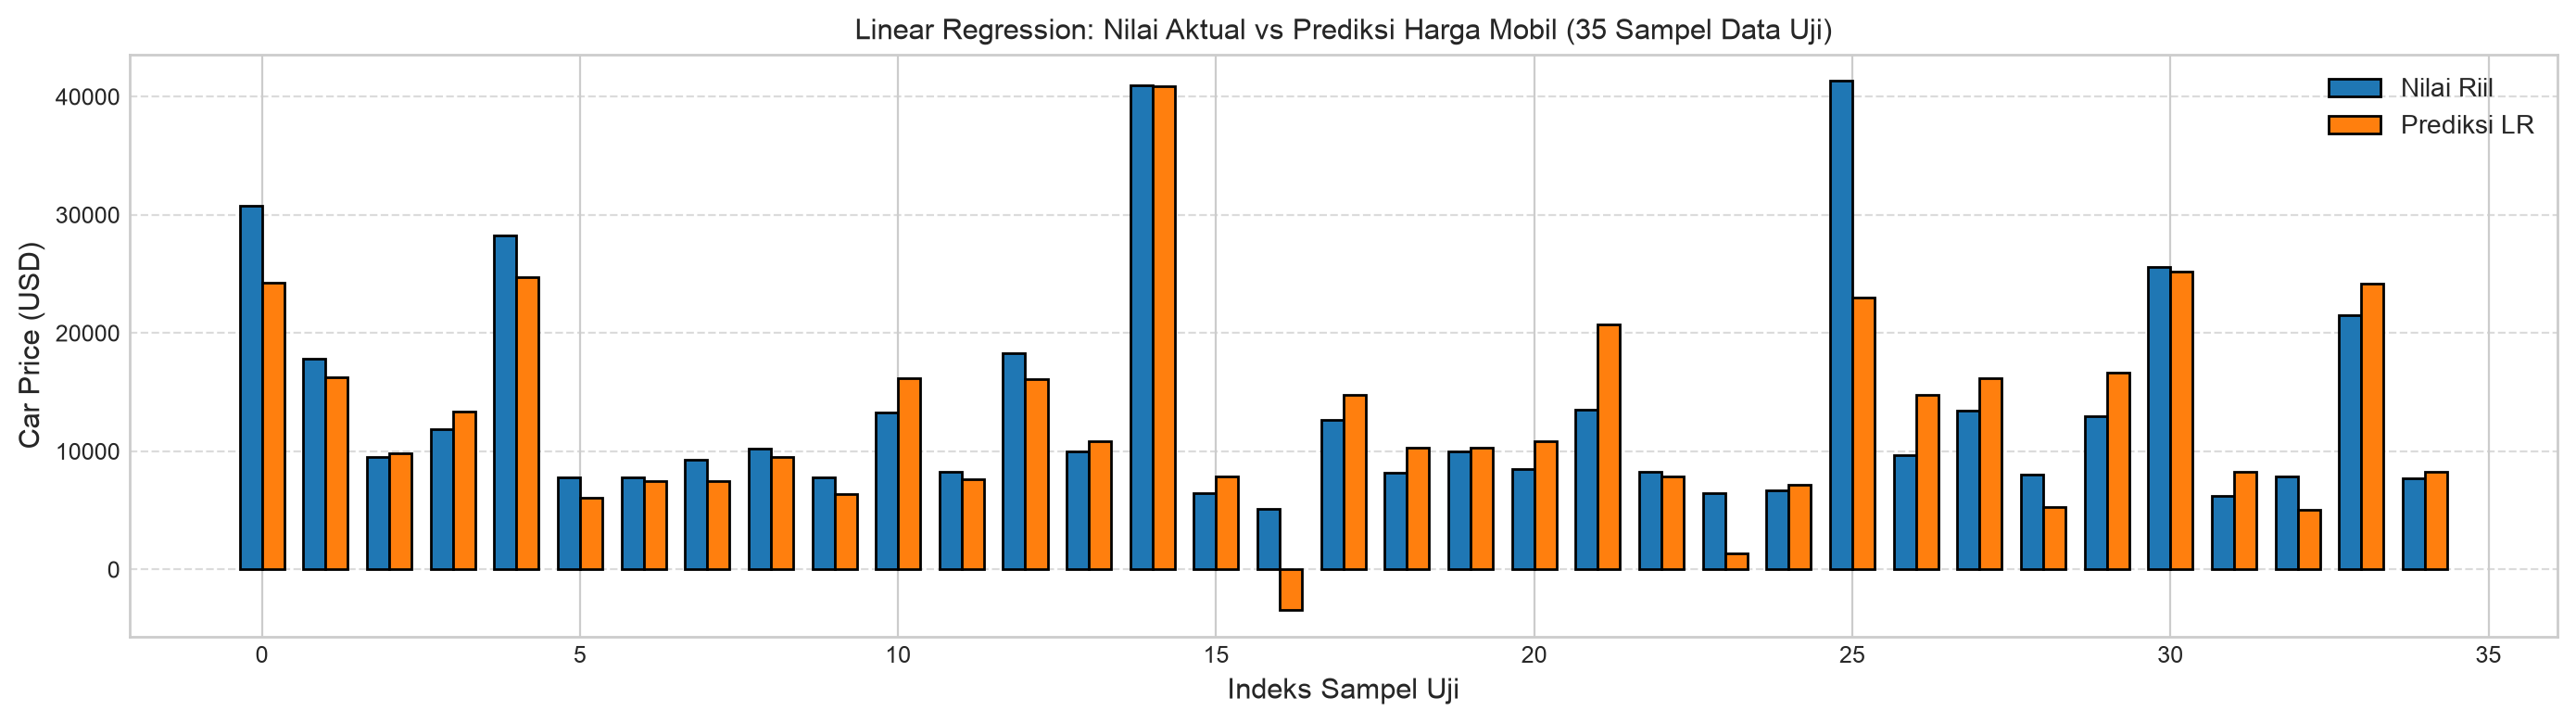
\includegraphics[width=\textwidth]{gambar/car_price_lr_comp.png}
    \vspace{0.2cm}
    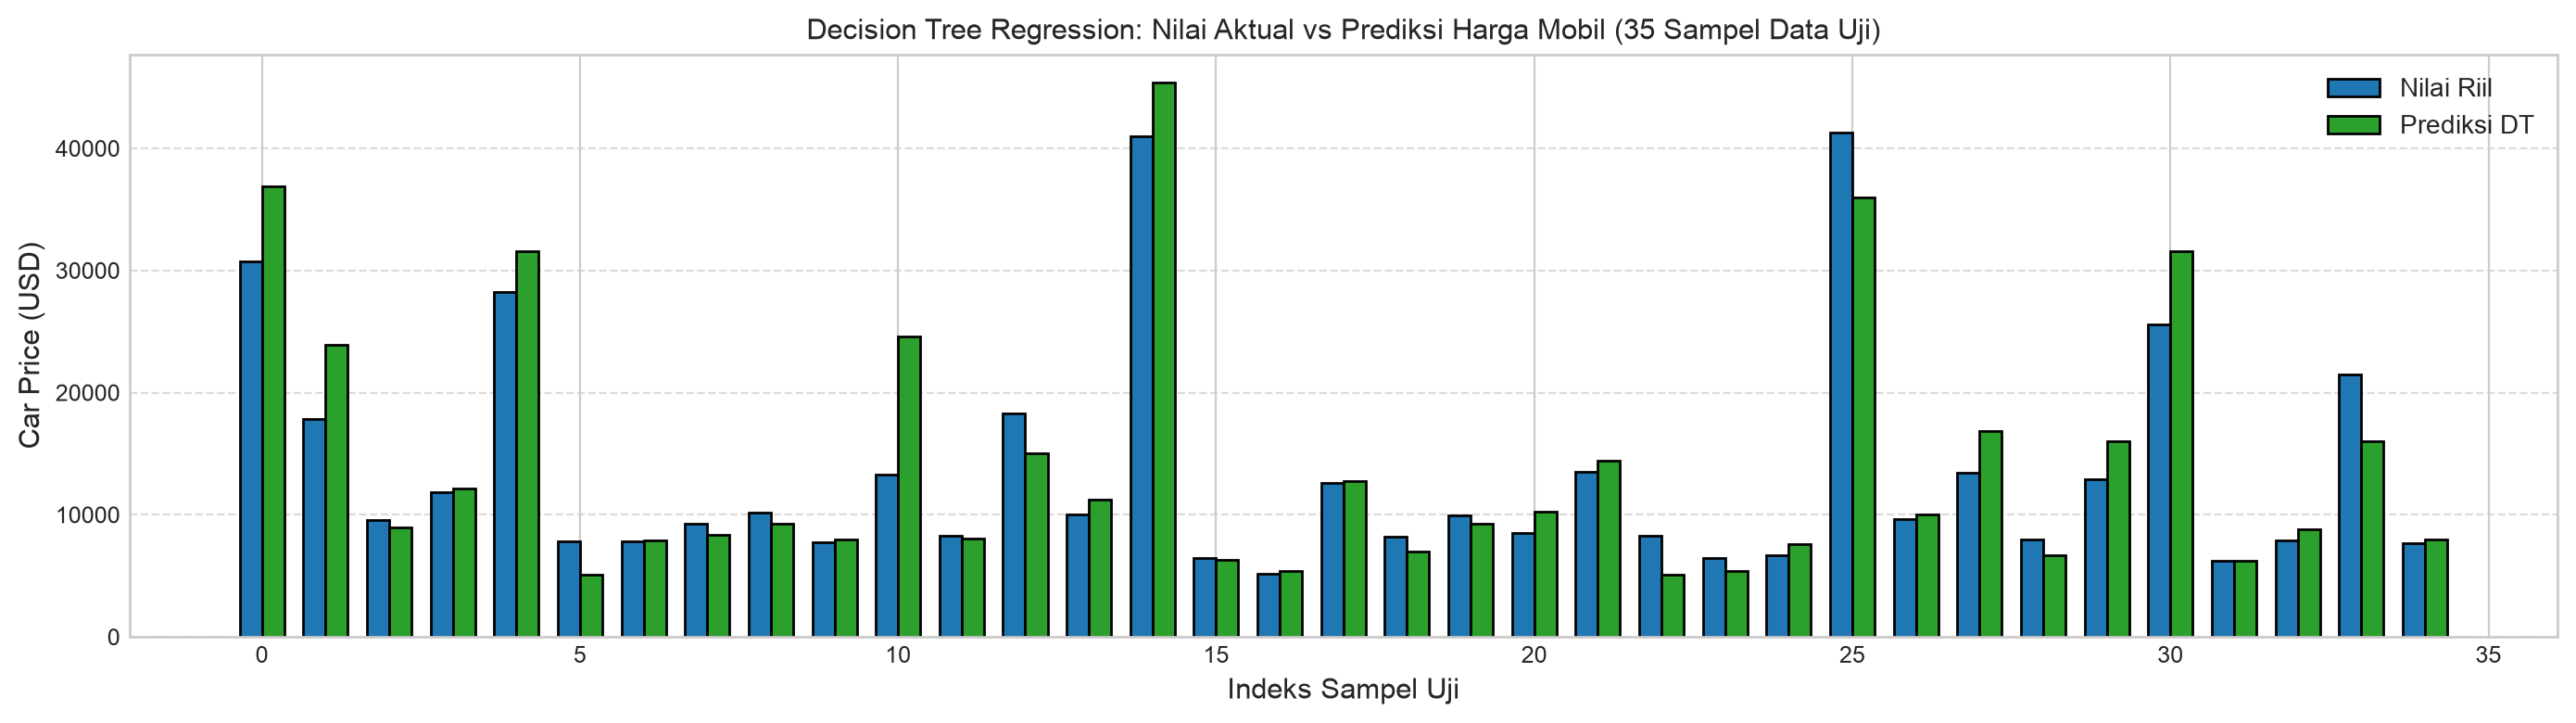
\includegraphics[width=\textwidth]{gambar/car_price_dt_comp.png}
    \vspace{0.2cm}
    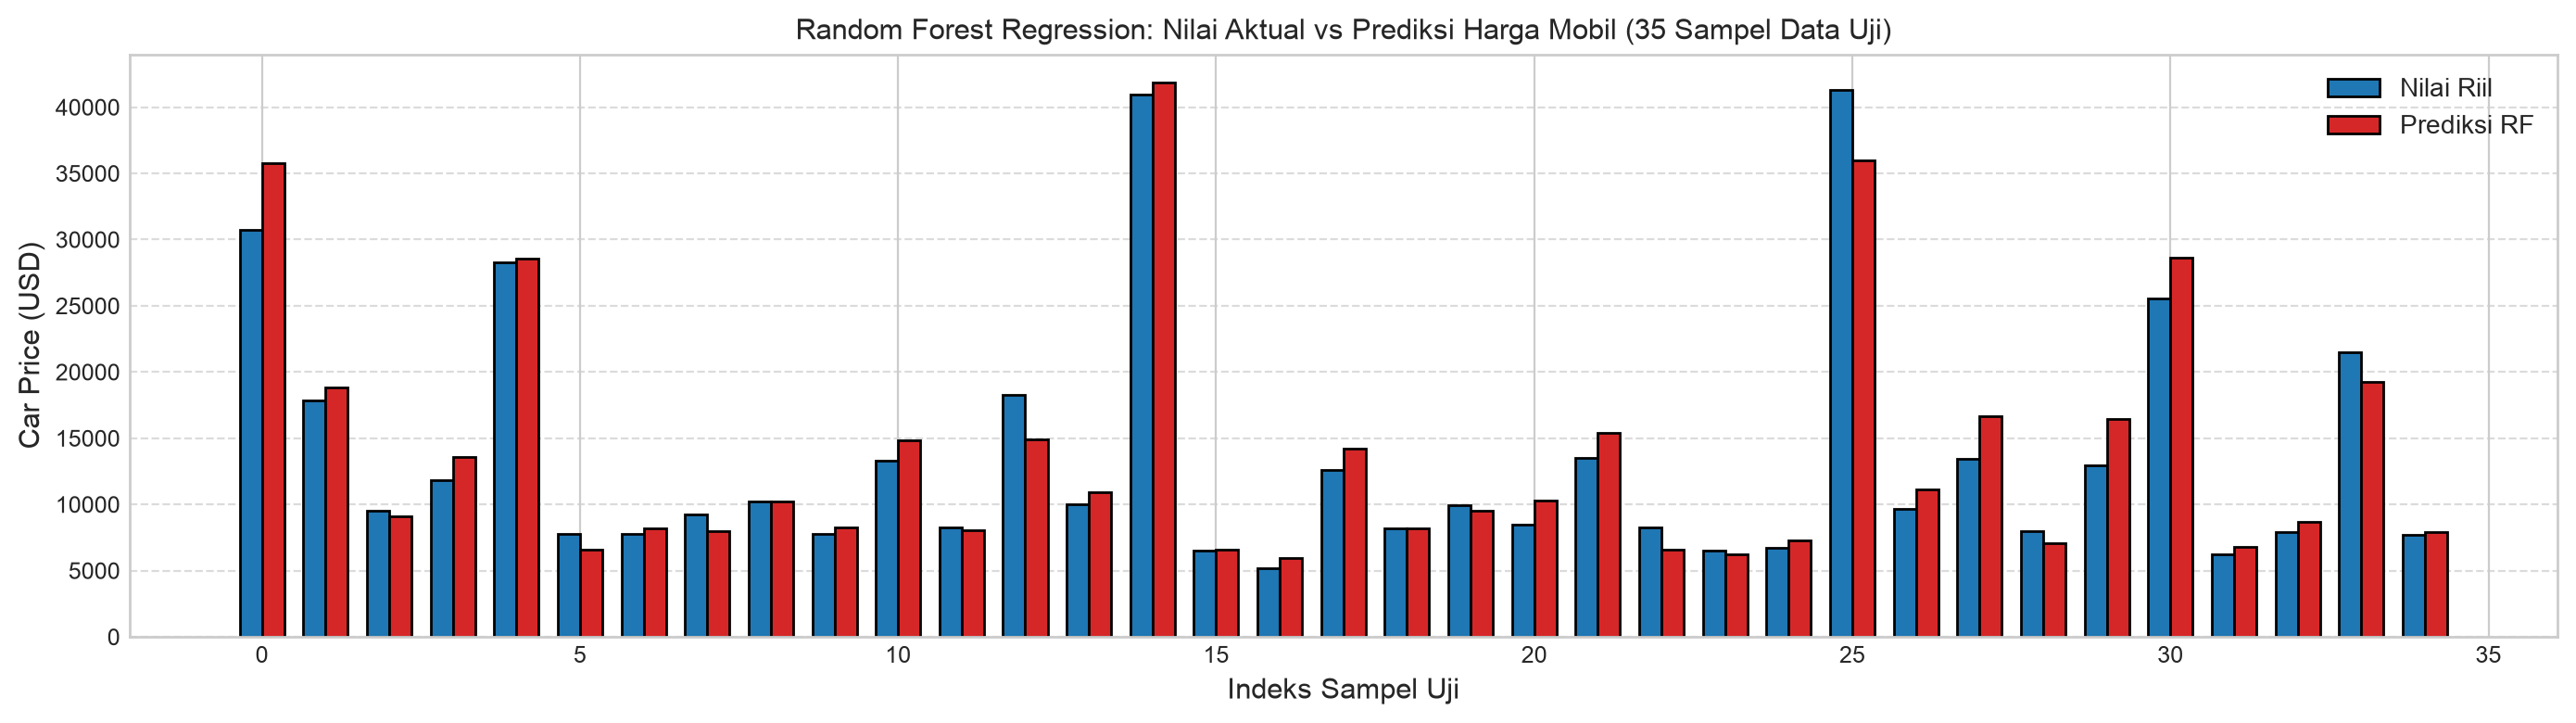
\includegraphics[width=\textwidth]{gambar/car_price_rf_comp.png}
    \caption{Perbandingan Nilai Aktual vs Prediksi pada 35 Sampel Data Uji Mobil untuk Linear Regression (atas), Decision Tree (tengah), dan Random Forest (bawah)}
    \label{fig:car_comp_grid}
\end{figure}

\subsection{Tabel Performa Model Machine Learning}
Hasil evaluasi performa yang membandingkan metrik RMSE, $R^2$, dan $R$ dari ketiga model regresi untuk kasus dataset harga mobil disajikan pada Gambar \ref{fig:colab-car-results-table} dan visualisasi diagram batang pada Gambar \ref{fig:car_price_metrics_comp}.

\screenshotimage[0.75\textwidth]{gambar/colab-car-results-table.png}{Tabel Ringkasan Performa Model Machine Learning pada Car Price Dataset di Google Colab}{colab-car-results-table}

\screenshotimage{gambar/car_price_metrics_comp.png}{Diagram Batang Komparasi Tiga Metrik Evaluasi (RMSE, $R^2$, $R$) pada Dataset Mobil}{car_price_metrics_comp}

\subsection{Analisis Model Terbaik}
Berdasarkan hasil evaluasi pemodelan pada Gambar \ref{fig:colab-car-results-table}, model \textbf{Random Forest Regression} terbukti menjadi model yang paling baik.

Pertimbangan dan alasan teknis pemilihan model ini didasarkan pada empat argumen berikut:

\begin{enumerate}
    \item \textbf{Galat Prediksi Terkecil (RMSE Terendah)}: \\
    Random Forest mencatatkan nilai RMSE sebesar 1955.87 USD. Angka ini jauh lebih kecil dibandingkan Decision Tree (2994.77 USD) dan Linear Regression (3722.33 USD). Penurunan nilai RMSE sebesar 1766.46 USD (turun 47.45\%) dibanding Linear Regression membuktikan bahwa rata-rata deviasi estimasi harga mobil oleh Random Forest jauh lebih presisi.

    \item \textbf{Daya Jelas Variansi Tertinggi ($R^2 = 0.9448$)}: \\
    Nilai koefisien determinasi Random Forest mencapai $0.9448$. Artinya, model mampu menerangkan 94.48\% dari total variabilitas harga mobil di dalam dataset pengujian. Sebaliknya, Linear Regression hanya mampu menjelaskan 80.00\% variansi data karena relasi non-linear antarspesifikasi mesin gagal ditangkap oleh model garis lurus.

    \item \textbf{Korelasi Estimasi Mendekati Sempurna ($R = 0.9727$)}: \\
    Nilai korelasi Pearson antara harga aktual dan hasil prediksi menyentuh angka 0.9727. Angka ini mencerminkan bahwa tren fluktuasi harga riil mobil diikuti secara sangat konsisten oleh keluaran model Random Forest tanpa mengalami deviasi arah prediksi.

    \item \textbf{Ketahanan Ansambel terhadap Resiko Overfitting}: \\
    Pohon keputusan tunggal (Decision Tree) rentan membentuk simpul keputusan yang terlalu spesifik pada data latih. Sebaliknya, Random Forest melatih sekumpulan pohon keputusan yang dibangun dari sampel \textit{bootstrap} dan subset fitur yang dipilih secara acak. Penggabungan banyak pohon melalui rata-rata prediksi (\textit{voting aggregation}) secara efektif meredam varians galat acak dan menghasilkan kemampuan generalisasi data baru yang sangat tangguh.
\end{enumerate}
\clearpage

%======================================================================
% BAB IV: KESIMPULAN
%======================================================================
\chapter{Kesimpulan}

Praktikum modul regresi ini membuktikan efektivitas pemodelan machine learning dalam memprediksi variabel target bertipe numerik kontinu, baik pada kasus penaksiran nilai properti hunian KC House Data maupun penentuan harga pasar kendaraan bermotor Car Price Prediction. Karakteristik matematis masing-masing algoritma menentukan ketepatan estimasi yang dihasilkan. Linear Regression menawarkan kecepatan komputasi dan kemudahan interpretasi bobot koefisien, namun model ini terbatas saat harus menangani relasi fitur yang bersifat non-linear atau rentan terdistorsi oleh titik pencilan data. Di sisi lain, Decision Tree Regression memiliki fleksibilitas tinggi dalam membentuk batas keputusan non-linear secara bertingkat, meski menyimpan kelemahan mendasar berupa kecenderungan overfitting apabila struktur kedalaman pohon tidak dibatasi melalui pemangkasan parameter.

Random Forest Regression secara konsisten membuktikan keunggulannya sebagai model terbaik pada seluruh rangkaian percobaan dan analisis tugas. Melalui mekanisme pembelajaran ansambel bootstrap aggregating, algoritma ini menggabungkan ratusan pohon keputusan acak sehingga mampu meredam varians galat dan menghasilkan estimasi yang stabil. Pada pengujian dataset Car Price Prediction, Random Forest mencatatkan margin galat terendah dengan RMSE sebesar 1955.87 USD, daya jelas variansi data $R^2$ tertinggi mencapai 0.9448, serta keselarasan korelasi Pearson $R$ sebesar 0.9727. Keberhasilan estimasi ini juga menegaskan pengaruh dominan dari fitur kapasitas silinder mesin, bobot total kendaraan, dan tenaga kuda mesin sebagai variabel pendorong utama kenaikan harga jual kendaraan, berbanding terbalik dengan tingkat efisiensi konsumsi bahan bakar.
\clearpage

%======================================================================
% DAFTAR PUSTAKA
%======================================================================
\begin{thebibliography}{99}
\addcontentsline{toc}{chapter}{Daftar Pustaka}

\bibitem{ref1}
Russell, S., \& Norvig, P. (2020). \textit{Artificial Intelligence: A Modern Approach} (4th ed.). Pearson.

\bibitem{ref4}
Han, J., Pei, J., \& Tong, H. (2022). \textit{Data Mining: Concepts and Techniques} (4th ed.). Morgan Kaufmann/Elsevier.

\bibitem{ref6}
Pedregosa, F., Varoquaux, G., Gramfort, A., Michel, V., Thirion, B., Grisel, O., Blondel, M., Prettenhofer, P., Weiss, R., Dubourg, V., Vanderplas, J., Passos, A., Cournapeau, D., Brucher, M., Perrot, M., \& Duchesnay, \'E. (2011). Scikit-learn: Machine Learning in Python. \textit{Journal of Machine Learning Research}, 12, 2825--2830.

\end{thebibliography}

\end{document}
